% Options for packages loaded elsewhere
\PassOptionsToPackage{unicode}{hyperref}
\PassOptionsToPackage{hyphens}{url}
%
\documentclass[
]{article}
\usepackage{amsmath,amssymb}
\usepackage{lmodern}
\usepackage{iftex}
\ifPDFTeX
  \usepackage[T1]{fontenc}
  \usepackage[utf8]{inputenc}
  \usepackage{textcomp} % provide euro and other symbols
\else % if luatex or xetex
  \usepackage{unicode-math}
  \defaultfontfeatures{Scale=MatchLowercase}
  \defaultfontfeatures[\rmfamily]{Ligatures=TeX,Scale=1}
\fi
% Use upquote if available, for straight quotes in verbatim environments
\IfFileExists{upquote.sty}{\usepackage{upquote}}{}
\IfFileExists{microtype.sty}{% use microtype if available
  \usepackage[]{microtype}
  \UseMicrotypeSet[protrusion]{basicmath} % disable protrusion for tt fonts
}{}
\makeatletter
\@ifundefined{KOMAClassName}{% if non-KOMA class
  \IfFileExists{parskip.sty}{%
    \usepackage{parskip}
  }{% else
    \setlength{\parindent}{0pt}
    \setlength{\parskip}{6pt plus 2pt minus 1pt}}
}{% if KOMA class
  \KOMAoptions{parskip=half}}
\makeatother
\usepackage{xcolor}
\usepackage[margin=2.54cm]{geometry}
\usepackage{graphicx}
\makeatletter
\def\maxwidth{\ifdim\Gin@nat@width>\linewidth\linewidth\else\Gin@nat@width\fi}
\def\maxheight{\ifdim\Gin@nat@height>\textheight\textheight\else\Gin@nat@height\fi}
\makeatother
% Scale images if necessary, so that they will not overflow the page
% margins by default, and it is still possible to overwrite the defaults
% using explicit options in \includegraphics[width, height, ...]{}
\setkeys{Gin}{width=\maxwidth,height=\maxheight,keepaspectratio}
% Set default figure placement to htbp
\makeatletter
\def\fps@figure{htbp}
\makeatother
\setlength{\emergencystretch}{3em} % prevent overfull lines
\providecommand{\tightlist}{%
  \setlength{\itemsep}{0pt}\setlength{\parskip}{0pt}}
\setcounter{secnumdepth}{-\maxdimen} % remove section numbering
\usepackage{booktabs}
\usepackage{caption}
\usepackage{longtable}
\ifLuaTeX
  \usepackage{selnolig}  % disable illegal ligatures
\fi
\IfFileExists{bookmark.sty}{\usepackage{bookmark}}{\usepackage{hyperref}}
\IfFileExists{xurl.sty}{\usepackage{xurl}}{} % add URL line breaks if available
\urlstyle{same} % disable monospaced font for URLs
\hypersetup{
  pdftitle={Analysis of power generation across USA in 2021},
  pdfauthor={Srishti Mutha, Sokna Kry, Samriddha Ghosh, Nagarajan Vaidya Subramanian},
  hidelinks,
  pdfcreator={LaTeX via pandoc}}

\title{Analysis of power generation across USA in 2021}
\author{Srishti Mutha, Sokna Kry, Samriddha Ghosh, Nagarajan Vaidya
Subramanian}
\date{Spring 2023}

\begin{document}
\maketitle

\tableofcontents 
\newpage
\listoftables 
\newpage
\listoffigures 
\newpage

\hypertarget{rationale-and-research-questions}{%
\subsubsection{Rationale and Research
Questions}\label{rationale-and-research-questions}}

The US has been transitioning towards a greater reliance on renewable
energy sources such as wind, solar, hydro power and many more
technologies. Analyzing the e-Grid data can provide insights into the
distribution of clean energy generation across US, performance of these
renewable energy sources, their impact on the electricity generation and
energy markets throughout USA, and whether they are meeting the
expectations of energy companies, policymakers, and consumers.

This project aims to use e-GRID 2021 (published January 2023) to answer
the following research questions:

\begin{enumerate}
\def\labelenumi{\arabic{enumi}.}
\tightlist
\item
  What is the distribution of electricity generation across the Bureau
  of Economic Analysis regions in the US, from both the renewable and
  non-renewable energy sources?
\item
  What is the distribution of generation from each type of renewable and
  non-renewable energy sources across Bureau of Economic Analysis
  regions in the US?
\item
  Greenhouse gas emissions across Bureau of Economic Analysis regions in
  the US from electricity generators.
\item
  Summary statistics of generators across the Bureau of Economic
  Analysis regions in the US, in terms of fuel source, nameplate
  capacity, annual net generation, and pollutants emitted?
\item
  Is there correlation between energy generators and pollutants emitted?
\end{enumerate}

These analyses will be performed by aggregating the states into
categories as done by the Bureau of Economic Analysis which divides the
states into 8 regions. We have added an additional ``Non-Contiguous''
category to represent states in the e-GRID dataset that are not part of
mainland USA.

\newpage

\hypertarget{dataset-information}{%
\subsubsection{Dataset Information}\label{dataset-information}}

The Emissions \& Generation Resource Integrated Database (e-GRID) is a
comprehensive source of data published by the Environment Protection
Agency of the US Government. This database describes various technical
and environmental parameters of all electric power plants in the US, and
is published annually. It includes emissions, emission rates,
generation, heat input, resource mix, and many other attributes. eGRID
is typically used for greenhouse gas registries and inventories, carbon
footprints, consumer information disclosure, emission inventories and
standards, power market changes, and avoided emission estimates.In our
project we have used the e-Grid 2021 data-set which was released on
January 30th, 2023.

Below are some summary statistics of the installed capacity and annual
generation per region, pollutants and their CO2 equivalents per region,
and lastly about the distribution of annual generation across different
renewable and non-renewable sources of energy.

\newpage

\hypertarget{exploratory-analysis}{%
\subsubsection{Exploratory Analysis}\label{exploratory-analysis}}

\newpage

\hypertarget{analysis}{%
\subsubsection{Analysis}\label{analysis}}

\hypertarget{question-1-what-is-the-distribution-of-electricity-generation-across-the-bureau-of-economic-analysis-regions-in-the-us-from-both-the-renewable-and-non-renewable-energy-sources}{%
\paragraph{Question 1: What is the distribution of electricity
generation across the Bureau of Economic Analysis regions in the US,
from both the renewable and non-renewable energy
sources?}\label{question-1-what-is-the-distribution-of-electricity-generation-across-the-bureau-of-economic-analysis-regions-in-the-us-from-both-the-renewable-and-non-renewable-energy-sources}}

The first research question focuses on the distribution of electricity
generation from renewable and non-renewable energy sources among the
Bureau of Economic Analysis (BEA) regions in the United States. The BEA
divides the United States into eight regions, which are:

\begin{enumerate}
\def\labelenumi{\arabic{enumi}.}
\tightlist
\item
  New England
\item
  Mideast
\item
  Great Lakes
\item
  Plains
\item
  Southeast
\item
  Southwest
\item
  Rocky Mountain
\item
  Far West
\end{enumerate}

The purpose of this question is to gain a deeper understanding of the
power production in different regions of the US and the types of energy
sources used. This data can aid policymakers and analysts in identifying
potential opportunities to increase the use of renewable energy sources
and decrease reliance on non-renewable sources, such as coal and natural
gas, which are known to contribute to greenhouse gas emissions and
climate change. Additionally, the data can assist companies and
investors in locating potential markets for renewable energy products
and services.

In order to determine the distribution of electricity generation across
the BEA regions in the USA, the states were grouped together based on
their respective regions. The state-wise annual electricity generation
was aggregated to obtain the region-wise annual generation. To better
visualize and compare the electricity generation across different
regions, we graphed the data in bar plots.

Figure 1: Distribution of Energy Sources by Region in 2021

\begin{center}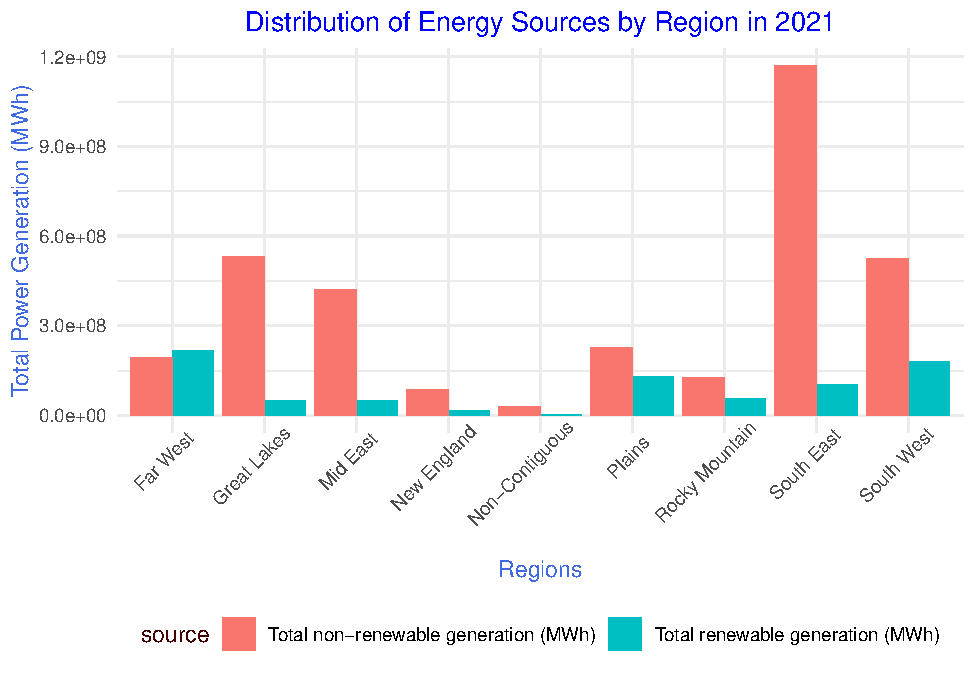
\includegraphics{EDA_Project_Mutha_Kry_Ghosh_VS_files/figure-latex/Q1plot-1} \end{center}

\hypertarget{question-2-what-is-the-distribution-of-generation-from-each-type-of-renewable-energy-sources-across-bureau-of-economic-analysis-regions-in-the-us}{%
\paragraph{Question 2: What is the distribution of generation from each
type of renewable energy sources across Bureau of Economic Analysis
regions in the
US?}\label{question-2-what-is-the-distribution-of-generation-from-each-type-of-renewable-energy-sources-across-bureau-of-economic-analysis-regions-in-the-us}}

The second research question looks deeper into the distribution of
electricity generation from each type of renewable energy source across
the BEA regions of the US. Renewable energy sources include solar, wind,
hydro, geothermal, and biomass.

The purpose of this question is to gain a better understanding of how
different regions in the United States are utilizing various renewable
energy sources for electricity generation. The data obtained can be
useful in identifying the potential for growth in the use of renewable
energy sources in certain regions and identifying areas where
investments in renewable energy infrastructure and technology may be
needed. It can be crucial data for policymakers to develop policies and
regulations that encourage the growth of specific renewable energy
across USA. The potential opportunities for growth and expansion of
renewable energy plants into regions that have high potential can also
be evaluated using this data. Additionally, this information can be
useful for identifying regions where investments in renewable energy
infrastructure could be profitable.

In order to determine the distribution of electricity generation from
each type of renewable energy sources across BEA regions in the US, the
states were grouped together based on their respective regions. The
state annual generation values for each type of renewable source were
aggregated to obtain the annual electricity generation. This enabled us
to obtain the total electricity generation for each type of renewable
energy source for each region, annually.

Figure 2: Distribution of different renewable energy generation sources
across BEA regions of USA in 2021

\begin{figure}

{\centering 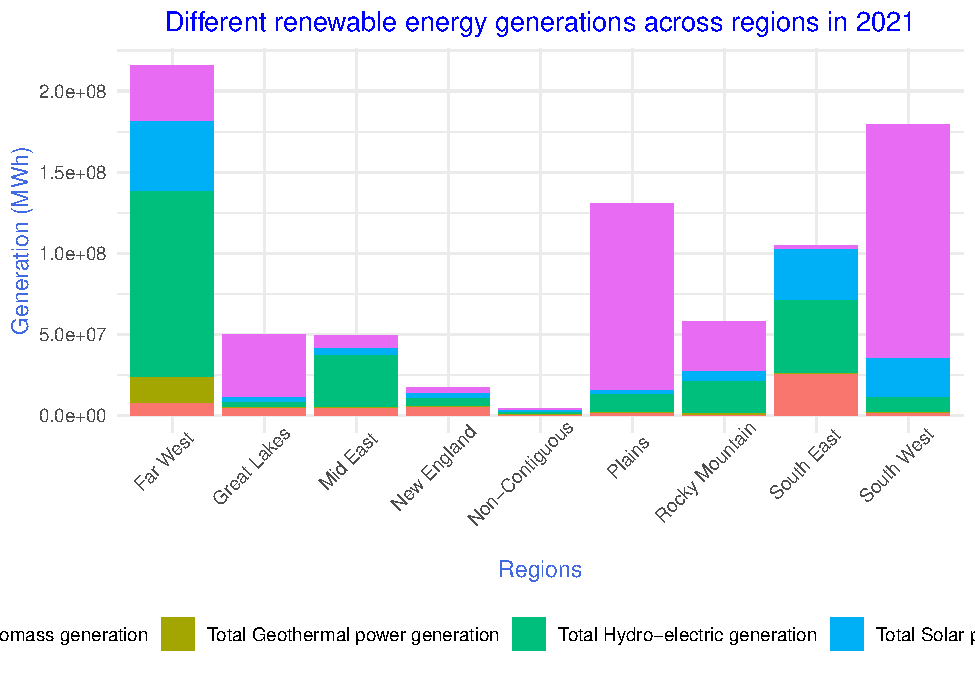
\includegraphics{EDA_Project_Mutha_Kry_Ghosh_VS_files/figure-latex/Q2plot-1} 

}

\caption{Different renewable energy generations across regions in 2021}\label{fig:Q2plot}
\end{figure}

\hypertarget{question-3-greenhouse-gas-emissions-across-bureau-of-economic-analysis-regions-in-the-us-from-electricity-generators.}{%
\paragraph{Question 3: Greenhouse gas emissions across Bureau of
Economic Analysis regions in the US from electricity
generators.}\label{question-3-greenhouse-gas-emissions-across-bureau-of-economic-analysis-regions-in-the-us-from-electricity-generators.}}

This question delves into greenhouse gas emissions from electricity
generators across the BEA regions in the US. Greenhouse gases, such as
carbon dioxide, methane, nitrous oxide, sulfur dioxide and many more are
released into the atmosphere as a result of the combustion of fossil
fuels for electricity generation, which contributes to climate change.

The purpose of this question is to understand the level of greenhouse
gas emissions from electricity generation in each region and to identify
areas where there may be opportunities to reduce greenhouse gas
emissions.

Analysts can make use of this data to gain insights into the sources and
levels of greenhouse gas emissions from electricity generators in each
region and help in the development of strategies for reducing emissions.
Policymakers across USA need this data to comprehend the necessity to
develop policies and regulations that encourage the transition to clean
energy sources and the reduction of greenhouse gas emissions from
electricity generators, such as carbon pricing or cap-and-trade
programs. This information is also crucial to identify regions where
investments in renewable energy infrastructure, technology and
operations may impact the environment.

In order to determine the greenhouse gas emissions across BEA regions in
the US from electricity generators,

Figure 3: Plot of total CO2 and CO2e emissions across BEA regions of USA
in 2021

\begin{figure}

{\centering 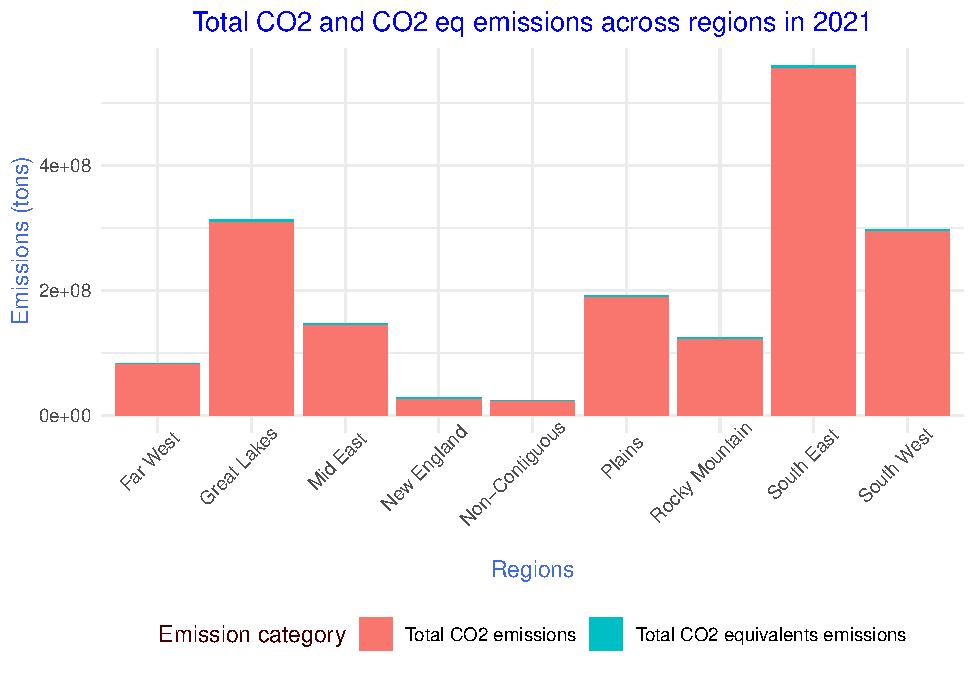
\includegraphics{EDA_Project_Mutha_Kry_Ghosh_VS_files/figure-latex/Q3plot-1} 

}

\caption{Total CO2 and CO2 eq emissions across regions in 2021}\label{fig:Q3plot}
\end{figure}

\hypertarget{question-4-summary-statistics-of-generators-across-the-bureau-of-economic-analysis-regions-in-the-us-in-terms-of-fuel-source-nameplate-capacity-annual-net-generation-and-pollutants-emitted}{%
\paragraph{Question 4: Summary statistics of generators across the
Bureau of Economic Analysis regions in the US, in terms of fuel source,
nameplate capacity, annual net generation, and pollutants
emitted}\label{question-4-summary-statistics-of-generators-across-the-bureau-of-economic-analysis-regions-in-the-us-in-terms-of-fuel-source-nameplate-capacity-annual-net-generation-and-pollutants-emitted}}

The summary statistics on electricity generators across the BEA regions
in the United States covers information such as the type of fuel source
used, the nameplate capacity of the generators, the annual net
generation of electricity, and the amount of pollutants emitted. We
performed some statistical analyses to obtain more insights. Boxplots
are used for summary statistics of this question as they are the most
appropriate visualization to understand the distribution of annual net
generation of electricity in different regions and the pollutants. They
provide a reliable way to compare medians, ranges, spread of data, and
identify potential outliers, and are more effective at communicating
this information than violin plots or scatter plots.

Looking at the plots for each region, we can see that the highest median
of pollutants is in the Great Lakes region, while the lowest is in New
England. Additionally, there is a potential outlier in the data for the
South West region.

obtain a comprehensive understanding of the electricity generation
infrastructure across different regions in the United States, to
facilitate the identification of opportunities for investment in
renewable energy infrastructure, evaluate the environmental impact of
electricity generation in each region, and to develop policies and
regulations that encourage the reduction of harmful emissions.

Figure 4: Carbon dioxide emissions in each BEA region in the USA in 2021

\begin{center}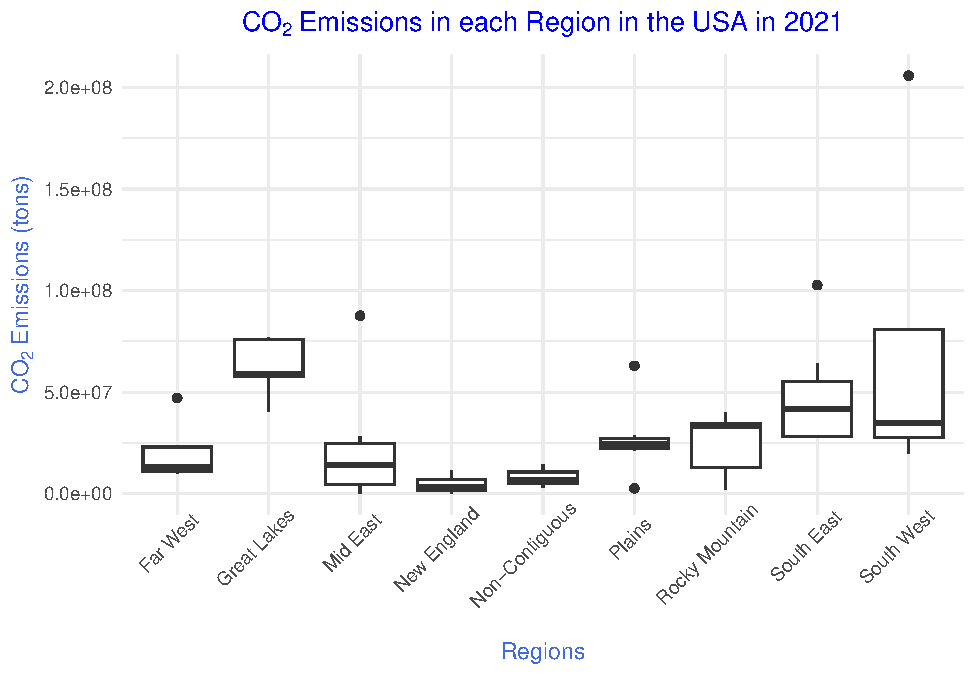
\includegraphics{EDA_Project_Mutha_Kry_Ghosh_VS_files/figure-latex/Q4plot_CO2-1} \end{center}

Figure 5: Sulfur dioxide emissions in each BEA region in the USA in 2021

\begin{center}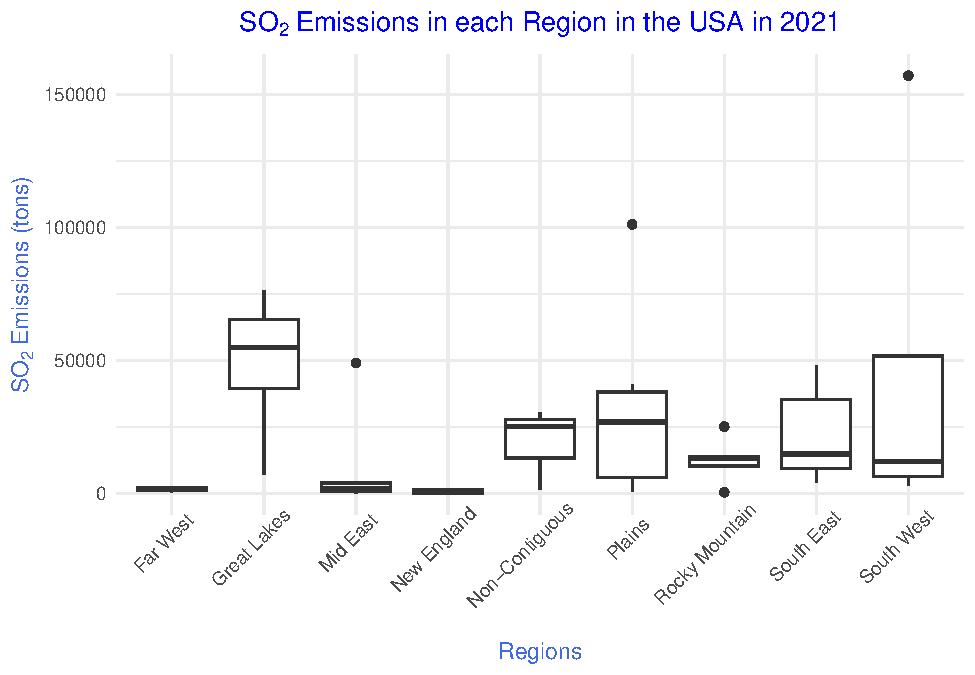
\includegraphics{EDA_Project_Mutha_Kry_Ghosh_VS_files/figure-latex/Q4plot_SO2-1} \end{center}

Figure 6: Nitrogen oxide emissions in each BEA region in the USA in 2021

\begin{center}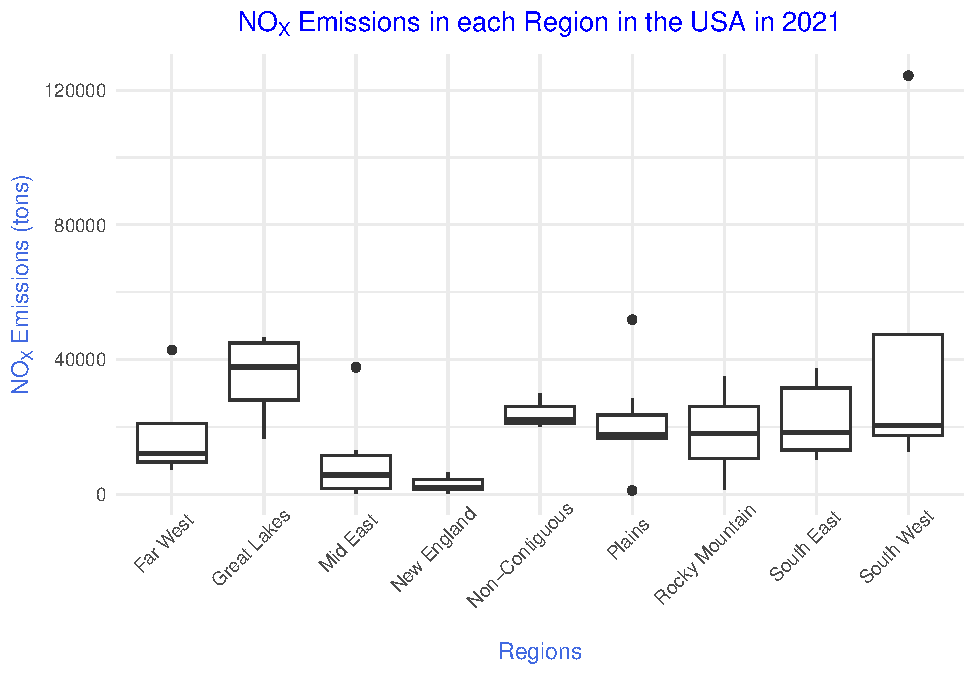
\includegraphics{EDA_Project_Mutha_Kry_Ghosh_VS_files/figure-latex/Q4plot_NOX-1} \end{center}

Figure 7: Carbon dioxide equivalent emissions in each BEA region in the
USA in 2021

\begin{center}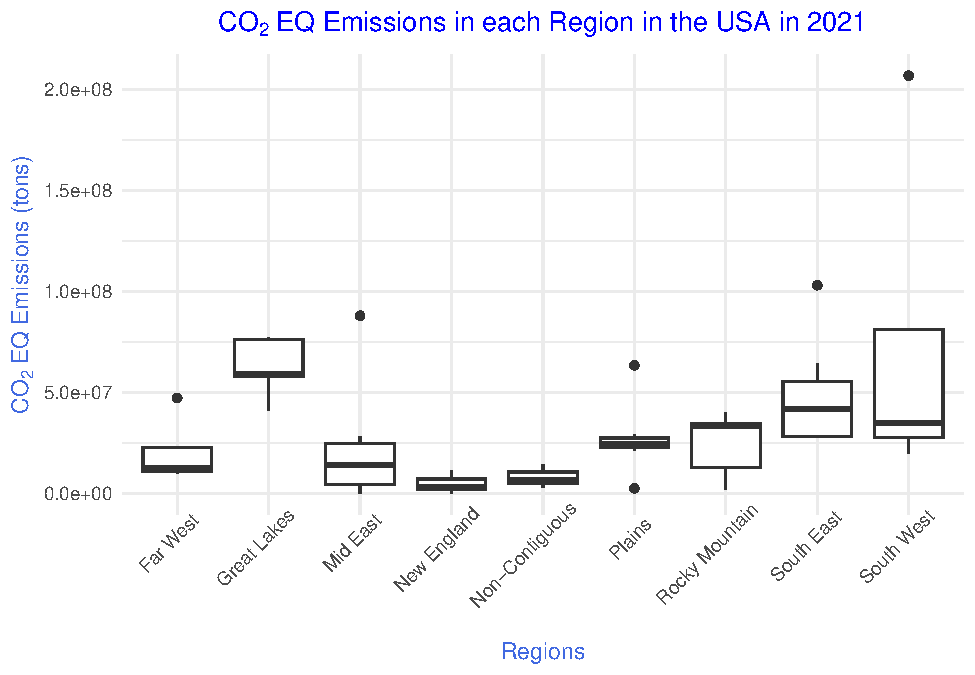
\includegraphics{EDA_Project_Mutha_Kry_Ghosh_VS_files/figure-latex/Q4plot_CO2e-1} \end{center}

\hypertarget{question-5-is-there-correlation-between-energy-generators-and-pollutants-emitted}{%
\paragraph{Question 5: Is there correlation between energy generators
and pollutants
emitted?}\label{question-5-is-there-correlation-between-energy-generators-and-pollutants-emitted}}

We wanted to understand the correlation between electricity generation
and the quantity of different pollutants that are emitted. First, we
developed linear regression models to understand the impact that
electricity generation has on the emissions of different pollutants (so
four linear regression models with one explanatory variable each). The
type of fuel source used by a generator affects the amount and type of
pollutants that are emitted during power generation. Power plants that
use non-renewable fuels such as coal, oil, and natural gas emit
pollutants such as carbon dioxide, methane, sulfur dioxide, nitrogen
oxides, and many more, majorly contribute to climate change and air
pollution.

Through this question we try to find this correlation between energy
generators and the pollutants they emit. The information can be used to
inform policy decisions related to reducing harmful emissions, such as
setting emissions standards or incentives to increase the use of cleaner
energy sources. It can also be useful for businesses to evaluate the
environmental impact of their operations and to identify opportunities
to reduce their carbon footprint. Understanding the correlation between
energy generators and pollutants emitted can provide insights into the
environmental impact of different types of energy sources and can be
used by energy analysts in models for predicting future emissions
trends.

The hypotheses for our models are as follows: \(H_o\): There is no
correlation between energy generation and pollutants emitted. \(H_a\):
There is some correlation between energy generation and pollutants
emitted.

The four models all had a p-value of \textless0.001 indicating that the
models had some explanatory power. We can therefore reject the null
hypothesis for all four models and conclude that there is some
correlation between energy generation and pollutants emitted.

Our models had different R2 values though. Annual electricity generation
is able to explain 63\% of the variance in NO\textsubscript{x} emissions
and only under 42\% of \(SO_2\) emissions. Whereas it explains 82\% of
the variance in emissions of \(CO_2\) and \(CO_2\)-equivalents. Further,
the \(\beta\) coefficients for the first two models (between electricity
generation and \(NO_x\) or \(SO_2\)) are of the order of \(10^{-4}\)
indicating a very small influence of electricity generation on the
quantity of pollutants emitted. Whereas the \(\beta\) coefficients for
the last two models (between electricity generation and \(CO_2\) or
\(CO_2\)-equivalents) are of the order of \(10^{-1}\) indicating that
electricity generation has a 1000-fold greater impact on \(CO_2\)
emissions than it does on the other pollutants we looked at.

\begin{verbatim}
## 
## Call:
## lm(formula = STNOXAN ~ STNGENAN, data = egrid_subset)
## 
## Residuals:
##    Min     1Q Median     3Q    Max 
## -19700  -7770  -2885   7305  31513 
## 
## Coefficients:
##              Estimate Std. Error t value Pr(>|t|)    
## (Intercept) 5.260e+03  2.389e+03   2.202   0.0323 *  
## STNGENAN    1.959e-04  2.125e-05   9.220  2.3e-12 ***
## ---
## Signif. codes:  0 '***' 0.001 '**' 0.01 '*' 0.05 '.' 0.1 ' ' 1
## 
## Residual standard error: 12220 on 50 degrees of freedom
## Multiple R-squared:  0.6296, Adjusted R-squared:  0.6222 
## F-statistic:    85 on 1 and 50 DF,  p-value: 2.3e-12
\end{verbatim}

\begin{verbatim}
## [1] "************************************************************"
\end{verbatim}

\begin{verbatim}
## 
## Call:
## lm(formula = STSO2AN ~ STNGENAN, data = egrid_subset)
## 
## Residuals:
##    Min     1Q Median     3Q    Max 
## -47341 -12377  -5099  13227  80726 
## 
## Coefficients:
##              Estimate Std. Error t value Pr(>|t|)    
## (Intercept) 2.342e+03  4.443e+03   0.527      0.6    
## STNGENAN    2.361e-04  3.952e-05   5.974  2.4e-07 ***
## ---
## Signif. codes:  0 '***' 0.001 '**' 0.01 '*' 0.05 '.' 0.1 ' ' 1
## 
## Residual standard error: 22730 on 50 degrees of freedom
## Multiple R-squared:  0.4165, Adjusted R-squared:  0.4048 
## F-statistic: 35.69 on 1 and 50 DF,  p-value: 2.4e-07
\end{verbatim}

\begin{verbatim}
## [1] "************************************************************"
\end{verbatim}

\begin{verbatim}
## 
## Call:
## lm(formula = STCO2AN ~ STNGENAN, data = egrid_subset)
## 
## Residuals:
##       Min        1Q    Median        3Q       Max 
## -34801066  -7155462  -2868586   4846472  37306906 
## 
## Coefficients:
##              Estimate Std. Error t value Pr(>|t|)    
## (Intercept) 3.106e+06  2.875e+06   1.081    0.285    
## STNGENAN    3.870e-01  2.557e-02  15.133   <2e-16 ***
## ---
## Signif. codes:  0 '***' 0.001 '**' 0.01 '*' 0.05 '.' 0.1 ' ' 1
## 
## Residual standard error: 14710000 on 50 degrees of freedom
## Multiple R-squared:  0.8208, Adjusted R-squared:  0.8172 
## F-statistic:   229 on 1 and 50 DF,  p-value: < 2.2e-16
\end{verbatim}

\begin{verbatim}
## [1] "************************************************************"
\end{verbatim}

\begin{verbatim}
## 
## Call:
## lm(formula = STCO2EQA ~ STNGENAN, data = egrid_subset)
## 
## Residuals:
##       Min        1Q    Median        3Q       Max 
## -34977547  -7210908  -2931564   4817282  37582130 
## 
## Coefficients:
##              Estimate Std. Error t value Pr(>|t|)    
## (Intercept) 3.163e+06  2.896e+06   1.092     0.28    
## STNGENAN    3.886e-01  2.576e-02  15.085   <2e-16 ***
## ---
## Signif. codes:  0 '***' 0.001 '**' 0.01 '*' 0.05 '.' 0.1 ' ' 1
## 
## Residual standard error: 14820000 on 50 degrees of freedom
## Multiple R-squared:  0.8199, Adjusted R-squared:  0.8162 
## F-statistic: 227.5 on 1 and 50 DF,  p-value: < 2.2e-16
\end{verbatim}

\begin{verbatim}
## [1] "************************************************************"
\end{verbatim}

Figure 8: Linear Regression plot of Annual Net Energy Generation and CO2
emissions

\begin{verbatim}
## `geom_smooth()` using formula = 'y ~ x'
\end{verbatim}

\begin{center}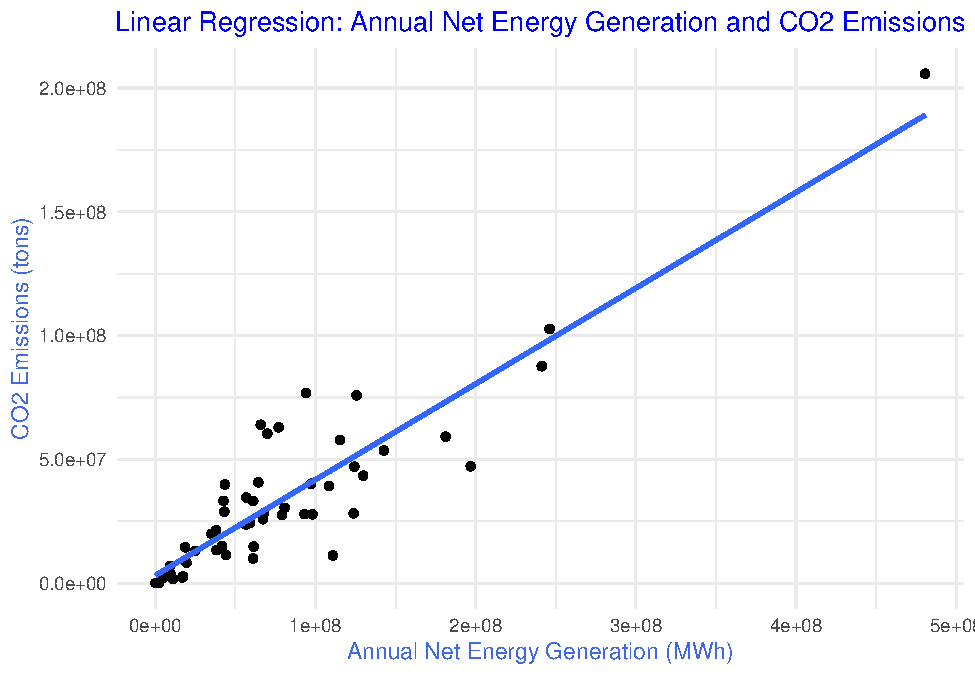
\includegraphics{EDA_Project_Mutha_Kry_Ghosh_VS_files/figure-latex/Q5_CO2-1} \end{center}

Figure 9: Linear Regression plot of Annual Net Energy Generation and
CO2e emissions

\begin{verbatim}
## `geom_smooth()` using formula = 'y ~ x'
\end{verbatim}

\begin{center}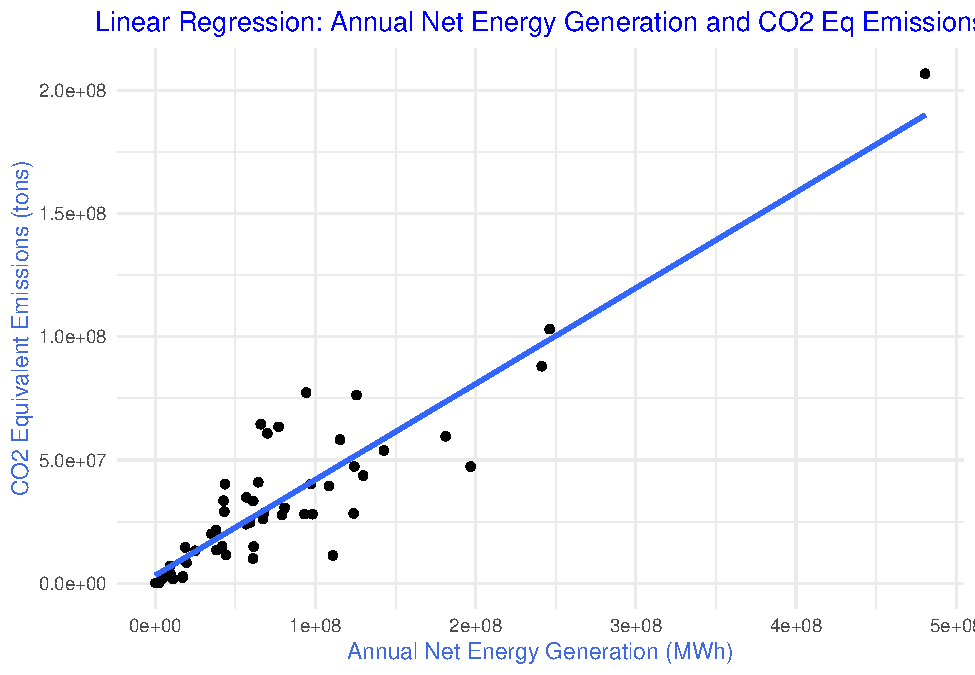
\includegraphics{EDA_Project_Mutha_Kry_Ghosh_VS_files/figure-latex/Q5_CO2e-1} \end{center}

Figure 10: Linear Regression plot of Annual Net Energy Generation and
SO2 emissions

\begin{verbatim}
## `geom_smooth()` using formula = 'y ~ x'
\end{verbatim}

\begin{center}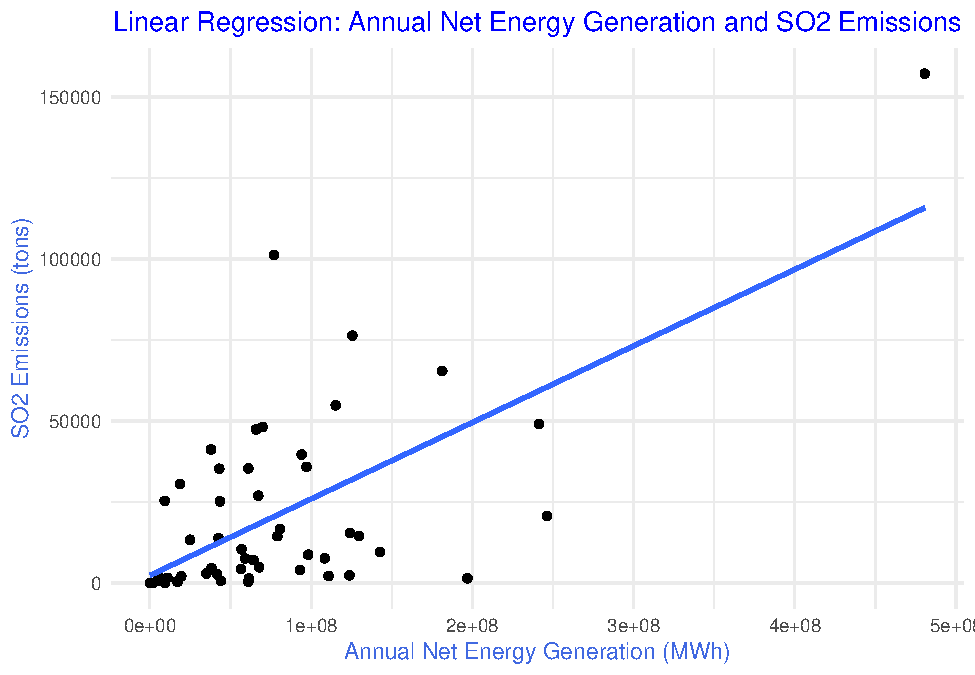
\includegraphics{EDA_Project_Mutha_Kry_Ghosh_VS_files/figure-latex/Q5_SO2-1} \end{center}

Figure 11: Linear Regression plot of Annual Net Energy Generation and
NOX emissions

\begin{verbatim}
## `geom_smooth()` using formula = 'y ~ x'
\end{verbatim}

\begin{center}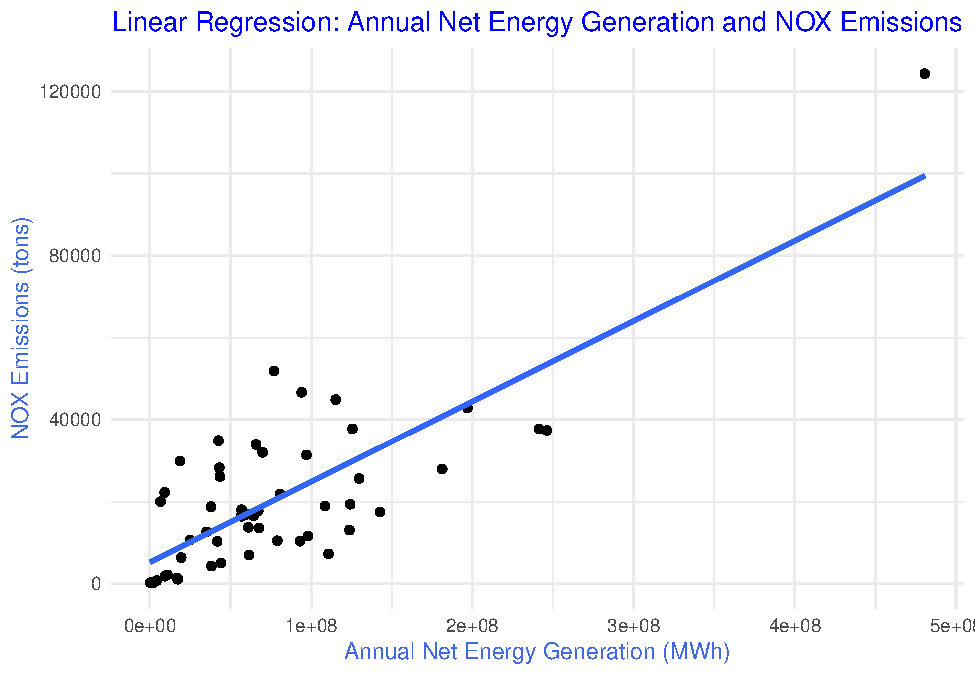
\includegraphics{EDA_Project_Mutha_Kry_Ghosh_VS_files/figure-latex/Q5_NOX-1} \end{center}

To build on this idea, we wanted to analyse the effects of different
parameters on the health of people in different states, we developed
three multiple linear regression models. They look at the effect that
the consumption of renewable energy has on people's health at the state
level instead of the region level so as to get more granular
information. We chose the following control variables: 1. air quality
(which can make people vulnerable to airborne illnesses), 2. education
level (which influences people's awareness of diseases and pollutants),
3. sex ratio (to separate out the predisposition of people of different
sex to have different exposures to occupational hazards), and 4. median
household income (which affects people's abilities to pay for
healthcare)

Figure 12: Plot showing the correlation between explanatory and response
variables for Model 1

\begin{verbatim}
## 
## Call:
## lm(formula = DeathRate ~ medianAQI + medianHHI + pctRene + pctEducation + 
##     SexRatio, data = dataset_final)
## 
## Residuals:
##     Min      1Q  Median      3Q     Max 
## -323.54  -38.26   25.17   54.24  336.93 
## 
## Coefficients:
##                Estimate Std. Error t value Pr(>|t|)    
## (Intercept)   2.356e+03  5.572e+02   4.228 0.000114 ***
## medianAQI     5.883e+00  2.675e+00   2.199 0.033029 *  
## medianHHI    -8.199e-03  1.439e-03  -5.696  8.8e-07 ***
## pctRene       7.127e+00  7.900e+01   0.090 0.928520    
## pctEducation  2.259e+03  5.702e+02   3.961 0.000263 ***
## SexRatio     -1.746e+01  6.469e+00  -2.699 0.009753 ** 
## ---
## Signif. codes:  0 '***' 0.001 '**' 0.01 '*' 0.05 '.' 0.1 ' ' 1
## 
## Residual standard error: 114.4 on 45 degrees of freedom
## Multiple R-squared:  0.6327, Adjusted R-squared:  0.5919 
## F-statistic:  15.5 on 5 and 45 DF,  p-value: 7.421e-09
\end{verbatim}

\begin{center}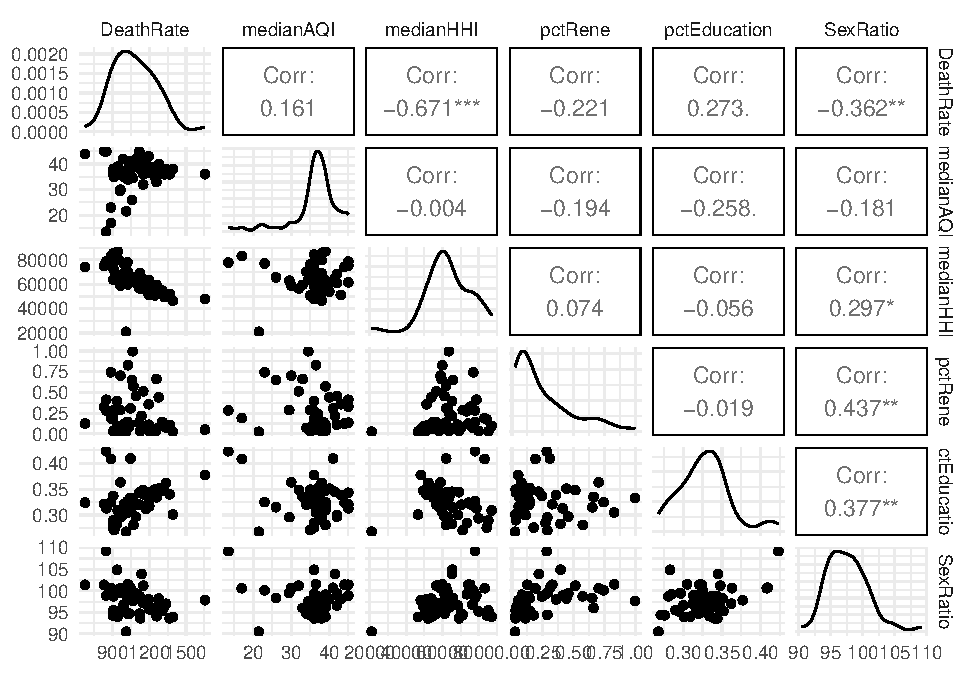
\includegraphics{EDA_Project_Mutha_Kry_Ghosh_VS_files/figure-latex/model1 results-1} \end{center}

This model has an F-statistic of 15.5 on 5 variables and 45 degrees of
freedom, corresponding to a p-value of \textless0.001. This indicates
that we can reject the null hypothesis and conclude that this model has
some explanatory power. This set of explanatory variables is able to
explain around 63\% of the variance in death rate across the US.

The correlation plot shows that we have some clustering of three
explanatory variables - median AQI, percentage of total generation from
renewables, and sex ratio. To improve the model we explored two
transformations for these clustered variables - one being rank-transform
and the other being log-transform.

Figure 13: Plot showing the correlation between explanatory and response
variables for Model 2

\begin{verbatim}
## 
## Call:
## lm(formula = DeathRate ~ rank_medianAQI + medianHHI + rank_pctRene + 
##     pctEducation + rank_SexRatio, data = model2_subset)
## 
## Residuals:
##     Min      1Q  Median      3Q     Max 
## -394.49  -46.50   22.73   63.68  364.36 
## 
## Coefficients:
##                  Estimate Std. Error t value Pr(>|t|)    
## (Intercept)     1.074e+03  2.074e+02   5.178 5.08e-06 ***
## rank_medianAQI  1.411e+00  1.147e+00   1.230 0.225110    
## medianHHI      -8.574e-03  1.419e-03  -6.044 2.69e-07 ***
## rank_pctRene    5.550e-02  1.502e+00   0.037 0.970691    
## pctEducation    1.912e+03  5.419e+02   3.528 0.000979 ***
## rank_SexRatio  -4.248e+00  1.585e+00  -2.680 0.010249 *  
## ---
## Signif. codes:  0 '***' 0.001 '**' 0.01 '*' 0.05 '.' 0.1 ' ' 1
## 
## Residual standard error: 116.6 on 45 degrees of freedom
## Multiple R-squared:  0.6186, Adjusted R-squared:  0.5762 
## F-statistic:  14.6 on 5 and 45 DF,  p-value: 1.681e-08
\end{verbatim}

\begin{center}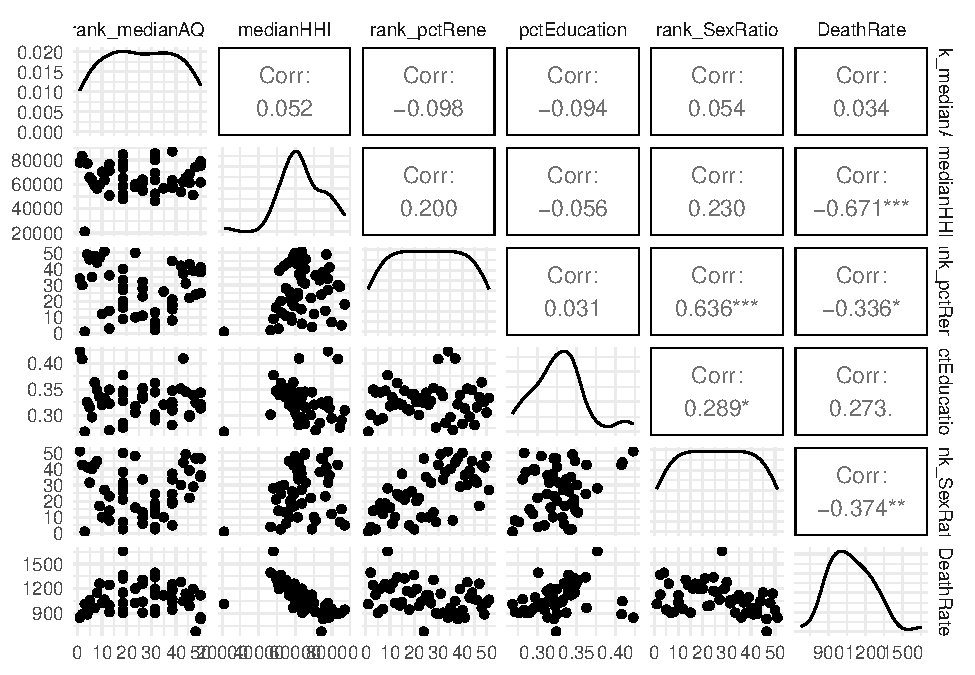
\includegraphics{EDA_Project_Mutha_Kry_Ghosh_VS_files/figure-latex/model2 results-1} \end{center}

Using the rank-transformed variables in our model, we get an F-statistic
of 14.6 on 5 variables and 45 degrees of freedom, corresponding to a
p-value \textless0.001. This means we can reject the null hypothesis for
this model and conclude it has some explanatory power. Looking at the R2
value, we see these explanatory variables can explain under 62\%

Figure 14: Plot showing the correlation between explanatory and response
variables for Model 3

\begin{verbatim}
## 
## Call:
## lm(formula = DeathRate ~ log_medianAQI + medianHHI + log_pctRene + 
##     pctEducation + log_SexRatio, data = model3_subset)
## 
## Residuals:
##     Min      1Q  Median      3Q     Max 
## -304.86  -36.56   22.78   55.65  322.70 
## 
## Coefficients:
##                 Estimate Std. Error t value Pr(>|t|)    
## (Intercept)    6.625e+03  3.123e+03   2.121 0.039445 *  
## log_medianAQI  1.966e+02  7.516e+01   2.616 0.012070 *  
## medianHHI     -8.122e-03  1.409e-03  -5.763 7.02e-07 ***
## log_pctRene   -8.111e+00  1.960e+01  -0.414 0.681042    
## pctEducation   2.287e+03  5.634e+02   4.059 0.000194 ***
## log_SexRatio  -1.417e+03  6.903e+02  -2.053 0.045945 *  
## ---
## Signif. codes:  0 '***' 0.001 '**' 0.01 '*' 0.05 '.' 0.1 ' ' 1
## 
## Residual standard error: 112.5 on 45 degrees of freedom
## Multiple R-squared:  0.6449, Adjusted R-squared:  0.6055 
## F-statistic: 16.35 on 5 and 45 DF,  p-value: 3.56e-09
\end{verbatim}

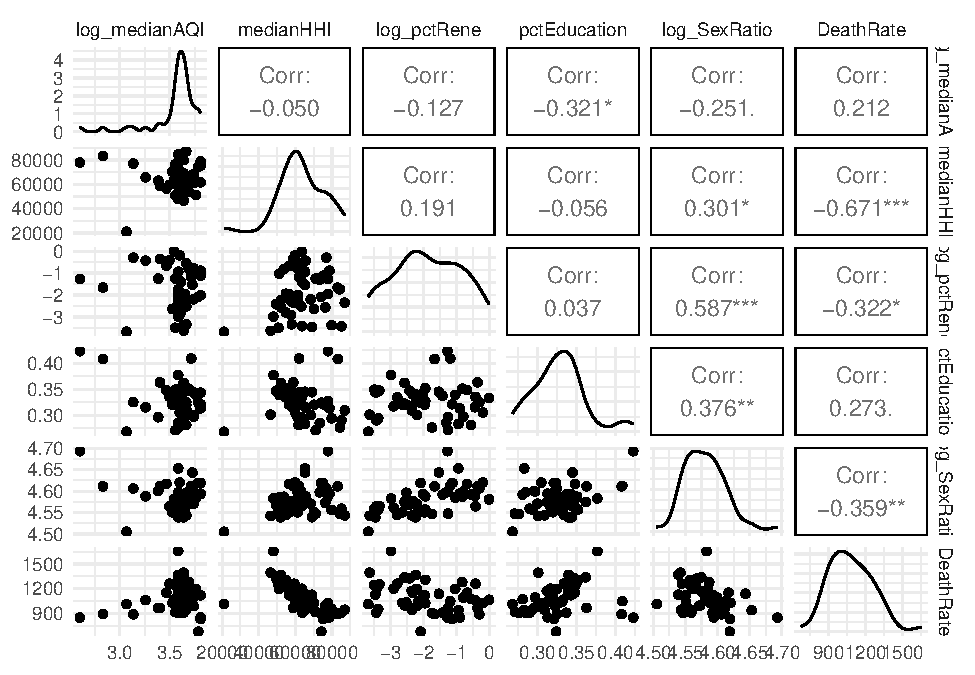
\includegraphics{EDA_Project_Mutha_Kry_Ghosh_VS_files/figure-latex/model3 results-1.pdf}

\newpage

\hypertarget{summary-and-conclusions}{%
\subsubsection{Summary and Conclusions}\label{summary-and-conclusions}}

\newpage

\hypertarget{appendix}{%
\subsubsection{Appendix}\label{appendix}}

\begin{longtable}{lrrrrrrr}
\caption*{
{\large Table 1: Summary Statistics for Variables per Region}
} \\ 
\toprule
Variable & Number of States & Minimum & Maximum & Mean & Median & Standard Deviation & Skewness \\ 
\midrule
\multicolumn{8}{l}{Far West} \\ 
\midrule
State annual net generation (GWh) & $4$ & $40,000$ & $200,000$ & $100,000$ & $90,000$ & 69289.84 & 0.41 \\ 
State nameplate capacity (GW) & $4$ & $10$ & $90$ & $40$ & $20$ & 33.57 & 0.65 \\ 
\midrule
\multicolumn{8}{l}{Great Lakes} \\ 
\midrule
State annual net generation (GWh) & $5$ & $60,000$ & $200,000$ & $100,000$ & $100,000$ & 43340.70 & 0.31 \\ 
State nameplate capacity (GW) & $5$ & $20$ & $50$ & $30$ & $30$ & 11.66 & 0.30 \\ 
\midrule
\multicolumn{8}{l}{Mid East} \\ 
\midrule
State annual net generation (GWh) & $6$ & $200$ & $200,000$ & $80,000$ & $50,000$ & 91763.39 & 0.75 \\ 
State nameplate capacity (GW) & $6$ & $0.05$ & $50$ & $20$ & $20$ & 21.84 & 0.35 \\ 
\midrule
\multicolumn{8}{l}{New England} \\ 
\midrule
State annual net generation (GWh) & $6$ & $2,000$ & $40,000$ & $20,000$ & $10,000$ & 14540.51 & 0.83 \\ 
State nameplate capacity (GW) & $6$ & $0.9$ & $20$ & $7$ & $5$ & 5.51 & 0.45 \\ 
\midrule
\multicolumn{8}{l}{Non-Contiguous} \\ 
\midrule
State annual net generation (GWh) & $3$ & $7,000$ & $20,000$ & $10,000$ & $9,000$ & 6306.16 & 0.31 \\ 
State nameplate capacity (GW) & $3$ & $3$ & $6$ & $4$ & $3$ & 1.84 & 0.38 \\ 
\midrule
\multicolumn{8}{l}{Plains} \\ 
\midrule
State annual net generation (GWh) & $7$ & $20,000$ & $80,000$ & $50,000$ & $60,000$ & 20007.36 & -0.35 \\ 
State nameplate capacity (GW) & $7$ & $7$ & $20$ & $20$ & $20$ & 7.00 & -0.19 \\ 
\midrule
\multicolumn{8}{l}{Rocky Mountain} \\ 
\midrule
State annual net generation (GWh) & $5$ & $20,000$ & $60,000$ & $40,000$ & $40,000$ & 15952.02 & -0.07 \\ 
State nameplate capacity (GW) & $5$ & $5$ & $20$ & $10$ & $10$ & 5.86 & 0.59 \\ 
\midrule
\multicolumn{8}{l}{South East} \\ 
\midrule
State annual net generation (GWh) & $10$ & $60,000$ & $200,000$ & $100,000$ & $100,000$ & 51631.87 & 1.53 \\ 
State nameplate capacity (GW) & $10$ & $20$ & $70$ & $30$ & $30$ & 15.47 & 1.42 \\ 
\midrule
\multicolumn{8}{l}{South West} \\ 
\midrule
State annual net generation (GWh) & $4$ & $40,000$ & $500,000$ & $200,000$ & $90,000$ & 205164.83 & 0.70 \\ 
State nameplate capacity (GW) & $4$ & $10$ & $200$ & $60$ & $30$ & 63.30 & 0.70 \\ 
\bottomrule
\end{longtable}

\begin{longtable}{lrrrrrrr}
\toprule
Variable & Observations & Minimum & Maximum & Mean & Median & Standard Deviation & Skewness \\ 
\midrule
\multicolumn{8}{l}{Far West} \\ 
\midrule
State annual CO2 emissions (tons) & $4$ & $10,000,000$ & $50,000,000$ & $20,000,000$ & $10,000,000$ & 17704508.67 & 0.72 \\ 
State annual CO2 equivalent emissions (tons) & $4$ & $10,000,000$ & $50,000,000$ & $20,000,000$ & $10,000,000$ & 17756214.90 & 0.72 \\ 
State annual NOx emissions (tons) & $4$ & $7,000$ & $40,000$ & $20,000$ & $10,000$ & 16414.69 & 0.69 \\ 
State annual SO2 emissions (tons) & $4$ & $500$ & $3,000$ & $2,000$ & $2,000$ & 956.99 & -0.25 \\ 
\midrule
\multicolumn{8}{l}{Great Lakes} \\ 
\midrule
State annual CO2 emissions (tons) & $5$ & $40,000,000$ & $80,000,000$ & $60,000,000$ & $60,000,000$ & 14926766.87 & -0.24 \\ 
State annual CO2 equivalent emissions (tons) & $5$ & $40,000,000$ & $80,000,000$ & $60,000,000$ & $60,000,000$ & 15008406.43 & -0.25 \\ 
State annual NOx emissions (tons) & $5$ & $20,000$ & $50,000$ & $30,000$ & $40,000$ & 12557.01 & -0.36 \\ 
State annual SO2 emissions (tons) & $5$ & $7,000$ & $80,000$ & $50,000$ & $50,000$ & 26897.63 & -0.48 \\ 
\midrule
\multicolumn{8}{l}{Mid East} \\ 
\midrule
State annual CO2 emissions (tons) & $6$ & $60,000$ & $90,000,000$ & $20,000,000$ & $10,000,000$ & 32645559.66 & 1.08 \\ 
State annual CO2 equivalent emissions (tons) & $6$ & $60,000$ & $90,000,000$ & $20,000,000$ & $10,000,000$ & 32788416.75 & 1.08 \\ 
State annual NOx emissions (tons) & $6$ & $300$ & $40,000$ & $10,000$ & $6,000$ & 14106.50 & 1.05 \\ 
State annual SO2 emissions (tons) & $6$ & $3$ & $50,000$ & $10,000$ & $2,000$ & 19351.02 & 1.34 \\ 
\midrule
\multicolumn{8}{l}{New England} \\ 
\midrule
State annual CO2 emissions (tons) & $6$ & $40,000$ & $10,000,000$ & $5,000,000$ & $3,000,000$ & 4315570.13 & 0.45 \\ 
State annual CO2 equivalent emissions (tons) & $6$ & $50,000$ & $10,000,000$ & $5,000,000$ & $3,000,000$ & 4337858.32 & 0.45 \\ 
State annual NOx emissions (tons) & $6$ & $200$ & $6,000$ & $3,000$ & $2,000$ & 2384.81 & 0.41 \\ 
State annual SO2 emissions (tons) & $6$ & $20$ & $2,000$ & $800$ & $600$ & 841.65 & 0.41 \\ 
\midrule
\multicolumn{8}{l}{Non-Contiguous} \\ 
\midrule
State annual CO2 emissions (tons) & $3$ & $3,000,000$ & $10,000,000$ & $8,000,000$ & $7,000,000$ & 5824848.33 & 0.21 \\ 
State annual CO2 equivalent emissions (tons) & $3$ & $3,000,000$ & $10,000,000$ & $8,000,000$ & $7,000,000$ & 5841693.80 & 0.21 \\ 
State annual NOx emissions (tons) & $3$ & $20,000$ & $30,000$ & $20,000$ & $20,000$ & 5178.34 & 0.31 \\ 
State annual SO2 emissions (tons) & $3$ & $1,000$ & $30,000$ & $20,000$ & $30,000$ & 15476.55 & -0.34 \\ 
\midrule
\multicolumn{8}{l}{Plains} \\ 
\midrule
State annual CO2 emissions (tons) & $7$ & $3,000,000$ & $60,000,000$ & $30,000,000$ & $20,000,000$ & 17982769.31 & 0.76 \\ 
State annual CO2 equivalent emissions (tons) & $7$ & $3,000,000$ & $60,000,000$ & $30,000,000$ & $20,000,000$ & 18127162.28 & 0.77 \\ 
State annual NOx emissions (tons) & $7$ & $1,000$ & $50,000$ & $20,000$ & $20,000$ & 15556.54 & 0.73 \\ 
State annual SO2 emissions (tons) & $7$ & $600$ & $100,000$ & $30,000$ & $30,000$ & 34762.13 & 0.98 \\ 
\midrule
\multicolumn{8}{l}{Rocky Mountain} \\ 
\midrule
State annual CO2 emissions (tons) & $5$ & $2,000,000$ & $40,000,000$ & $20,000,000$ & $30,000,000$ & 16109439.03 & -0.36 \\ 
State annual CO2 equivalent emissions (tons) & $5$ & $2,000,000$ & $40,000,000$ & $20,000,000$ & $30,000,000$ & 16223253.72 & -0.36 \\ 
State annual NOx emissions (tons) & $5$ & $1,000$ & $30,000$ & $20,000$ & $20,000$ & 13045.94 & -0.01 \\ 
State annual SO2 emissions (tons) & $5$ & $500$ & $30,000$ & $10,000$ & $10,000$ & 8836.50 & 0.05 \\ 
\midrule
\multicolumn{8}{l}{South East} \\ 
\midrule
State annual CO2 emissions (tons) & $10$ & $30,000,000$ & $100,000,000$ & $50,000,000$ & $40,000,000$ & 21985361.63 & 1.25 \\ 
State annual CO2 equivalent emissions (tons) & $10$ & $30,000,000$ & $100,000,000$ & $50,000,000$ & $40,000,000$ & 22095901.66 & 1.25 \\ 
State annual NOx emissions (tons) & $10$ & $10,000$ & $40,000$ & $20,000$ & $20,000$ & 9903.01 & 0.27 \\ 
State annual SO2 emissions (tons) & $10$ & $4,000$ & $50,000$ & $20,000$ & $10,000$ & 15955.90 & 0.55 \\ 
\midrule
\multicolumn{8}{l}{South West} \\ 
\midrule
State annual CO2 emissions (tons) & $4$ & $20,000,000$ & $200,000,000$ & $70,000,000$ & $30,000,000$ & 88321933.65 & 0.73 \\ 
State annual CO2 equivalent emissions (tons) & $4$ & $20,000,000$ & $200,000,000$ & $70,000,000$ & $40,000,000$ & 88713493.71 & 0.73 \\ 
State annual NOx emissions (tons) & $4$ & $10,000$ & $100,000$ & $40,000$ & $20,000$ & 53389.76 & 0.74 \\ 
State annual SO2 emissions (tons) & $4$ & $3,000$ & $200,000$ & $50,000$ & $10,000$ & 74265.46 & 0.74 \\ 
\bottomrule
\end{longtable}

\begin{longtable}{lrrrrrrr}
\toprule
Variable & Observations & Minimum & Maximum & Mean & Median & Standard Deviation & Skewness \\ 
\midrule
\multicolumn{8}{l}{Far West} \\ 
\midrule
State annual biomass net generation (GWh) & $4$ & $50$ & $5,000$ & $2,000$ & $1,000$ & 2349.53 & 0.60 \\ 
State annual coal net generation (GWh) & $4$ & $0$ & $3,000$ & $2,000$ & $2,000$ & 1625.82 & 0.01 \\ 
State annual gas net generation (GWh) & $4$ & $20,000$ & $100,000$ & $40,000$ & $20,000$ & 38150.42 & 0.73 \\ 
State annual geothermal net generation (GWh) & $4$ & $0$ & $10,000$ & $4,000$ & $2,000$ & 5203.54 & 0.51 \\ 
State annual hydro net generation (GWh) & $4$ & $2,000$ & $70,000$ & $30,000$ & $20,000$ & 30244.89 & 0.49 \\ 
State annual nuclear net generation (GWh) & $4$ & $0$ & $20,000$ & $6,000$ & $4,000$ & 7912.80 & 0.30 \\ 
State annual oil net generation (GWh) & $4$ & $0.4$ & $80$ & $30$ & $20$ & 34.13 & 0.45 \\ 
State annual other fossil net generation (GWh) & $4$ & $0$ & $2,000$ & $500$ & $200$ & 725.63 & 0.68 \\ 
State annual solar net generation (GWh) & $4$ & $50$ & $30,000$ & $10,000$ & $4,000$ & 16322.85 & 0.69 \\ 
State annual wind net generation (GWh) & $4$ & $300$ & $20,000$ & $9,000$ & $9,000$ & 6125.44 & -0.28 \\ 
\midrule
\multicolumn{8}{l}{Great Lakes} \\ 
\midrule
State annual biomass net generation (GWh) & $5$ & $400$ & $2,000$ & $900$ & $600$ & 754.69 & 0.76 \\ 
State annual coal net generation (GWh) & $5$ & $30,000$ & $50,000$ & $40,000$ & $40,000$ & 10057.16 & -0.13 \\ 
State annual gas net generation (GWh) & $5$ & $20,000$ & $60,000$ & $30,000$ & $30,000$ & 14494.51 & 0.86 \\ 
State annual geothermal net generation (GWh) & $5$ & $0$ & $0$ & $0$ & $0$ & 0.00 & NaN \\ 
State annual hydro net generation (GWh) & $5$ & $100$ & $2,000$ & $800$ & $600$ & 791.56 & 0.91 \\ 
State annual nuclear net generation (GWh) & $5$ & $0$ & $100,000$ & $30,000$ & $20,000$ & 38566.53 & 0.81 \\ 
State annual oil net generation (GWh) & $5$ & $50$ & $1,000$ & $600$ & $300$ & 540.13 & 0.23 \\ 
State annual other fossil net generation (GWh) & $5$ & $30$ & $2,000$ & $900$ & $800$ & 904.52 & 0.37 \\ 
State annual solar net generation (GWh) & $5$ & $400$ & $700$ & $500$ & $500$ & 117.26 & 0.12 \\ 
State annual wind net generation (GWh) & $5$ & $2,000$ & $20,000$ & $8,000$ & $8,000$ & 6966.76 & 0.65 \\ 
\midrule
\multicolumn{8}{l}{Mid East} \\ 
\midrule
State annual biomass net generation (GWh) & $6$ & $60$ & $2,000$ & $800$ & $500$ & 827.19 & 0.37 \\ 
State annual coal net generation (GWh) & $6$ & $0$ & $30,000$ & $6,000$ & $700$ & 11581.28 & 1.28 \\ 
State annual gas net generation (GWh) & $6$ & $100$ & $100,000$ & $40,000$ & $20,000$ & 47806.43 & 0.89 \\ 
State annual geothermal net generation (GWh) & $6$ & $0$ & $0$ & $0$ & $0$ & 0.00 & NaN \\ 
State annual hydro net generation (GWh) & $6$ & $-100$ & $30,000$ & $5,000$ & $1,000$ & 11279.76 & 1.33 \\ 
State annual nuclear net generation (GWh) & $6$ & $0$ & $80,000$ & $30,000$ & $20,000$ & 28246.09 & 0.74 \\ 
State annual oil net generation (GWh) & $6$ & $0.04$ & $700$ & $200$ & $50$ & 261.24 & 1.28 \\ 
State annual other fossil net generation (GWh) & $6$ & $0$ & $1,000$ & $600$ & $500$ & 552.45 & 0.36 \\ 
State annual solar net generation (GWh) & $6$ & $20$ & $1,000$ & $600$ & $400$ & 562.22 & 0.32 \\ 
State annual wind net generation (GWh) & $6$ & $0$ & $4,000$ & $1,000$ & $300$ & 1918.42 & 0.55 \\ 
\midrule
\multicolumn{8}{l}{New England} \\ 
\midrule
State annual biomass net generation (GWh) & $6$ & $200$ & $2,000$ & $900$ & $800$ & 600.44 & 0.67 \\ 
State annual coal net generation (GWh) & $6$ & $0$ & $300$ & $100$ & $20$ & 132.11 & 0.51 \\ 
State annual gas net generation (GWh) & $6$ & $2$ & $20,000$ & $9,000$ & $7,000$ & 9044.24 & 0.57 \\ 
State annual geothermal net generation (GWh) & $6$ & $0$ & $0$ & $0$ & $0$ & 0.00 & NaN \\ 
State annual hydro net generation (GWh) & $6$ & $4$ & $3,000$ & $1,000$ & $900$ & 864.49 & 0.73 \\ 
State annual nuclear net generation (GWh) & $6$ & $0$ & $20,000$ & $5,000$ & $0$ & 7367.45 & 0.77 \\ 
State annual oil net generation (GWh) & $6$ & $3$ & $80$ & $40$ & $40$ & 31.14 & 0.09 \\ 
State annual other fossil net generation (GWh) & $6$ & $0$ & $900$ & $300$ & $100$ & 379.76 & 0.68 \\ 
State annual solar net generation (GWh) & $6$ & $4$ & $2,000$ & $400$ & $200$ & 565.29 & 1.26 \\ 
State annual wind net generation (GWh) & $6$ & $10$ & $3,000$ & $600$ & $300$ & 952.19 & 1.27 \\ 
\midrule
\multicolumn{8}{l}{Non-Contiguous} \\ 
\midrule
State annual biomass net generation (GWh) & $3$ & $0$ & $300$ & $100$ & $40$ & 153.38 & 0.36 \\ 
State annual coal net generation (GWh) & $3$ & $800$ & $3,000$ & $2,000$ & $1,000$ & 1360.30 & 0.36 \\ 
State annual gas net generation (GWh) & $3$ & $0$ & $8,000$ & $4,000$ & $3,000$ & 4005.06 & 0.14 \\ 
State annual geothermal net generation (GWh) & $3$ & $0$ & $200$ & $60$ & $0$ & 105.88 & 0.38 \\ 
State annual hydro net generation (GWh) & $3$ & $0$ & $2,000$ & $600$ & $100$ & 943.65 & 0.38 \\ 
State annual nuclear net generation (GWh) & $3$ & $0$ & $0$ & $0$ & $0$ & 0.00 & NaN \\ 
State annual oil net generation (GWh) & $3$ & $900$ & $7,000$ & $5,000$ & $6,000$ & 3271.75 & -0.36 \\ 
State annual other fossil net generation (GWh) & $3$ & $0$ & $200$ & $70$ & $0$ & 114.73 & 0.38 \\ 
State annual solar net generation (GWh) & $3$ & $0$ & $500$ & $300$ & $300$ & 254.83 & -0.14 \\ 
State annual wind net generation (GWh) & $3$ & $100$ & $700$ & $300$ & $200$ & 294.30 & 0.38 \\ 
\midrule
\multicolumn{8}{l}{Plains} \\ 
\midrule
State annual biomass net generation (GWh) & $7$ & $2$ & $1,000$ & $300$ & $90$ & 448.08 & 1.55 \\ 
State annual coal net generation (GWh) & $7$ & $2,000$ & $60,000$ & $20,000$ & $20,000$ & 17109.00 & 0.94 \\ 
State annual gas net generation (GWh) & $7$ & $1,000$ & $10,000$ & $5,000$ & $3,000$ & 4245.14 & 0.85 \\ 
State annual geothermal net generation (GWh) & $7$ & $0$ & $0$ & $0$ & $0$ & 0.00 & NaN \\ 
State annual hydro net generation (GWh) & $7$ & $30$ & $5,000$ & $2,000$ & $1,000$ & 1608.68 & 1.10 \\ 
State annual nuclear net generation (GWh) & $7$ & $0$ & $10,000$ & $5,000$ & $4,000$ & 5398.44 & 0.47 \\ 
State annual oil net generation (GWh) & $7$ & $30$ & $300$ & $100$ & $100$ & 79.83 & 0.66 \\ 
State annual other fossil net generation (GWh) & $7$ & $0$ & $300$ & $40$ & $0$ & 95.42 & 1.51 \\ 
State annual solar net generation (GWh) & $7$ & $0$ & $2,000$ & $300$ & $60$ & 685.93 & 1.58 \\ 
State annual wind net generation (GWh) & $7$ & $7,000$ & $40,000$ & $20,000$ & $10,000$ & 11004.37 & 0.83 \\ 
\midrule
\multicolumn{8}{l}{Rocky Mountain} \\ 
\midrule
State annual biomass net generation (GWh) & $5$ & $0$ & $500$ & $200$ & $80$ & 197.08 & 0.82 \\ 
State annual coal net generation (GWh) & $5$ & $20$ & $30,000$ & $20,000$ & $20,000$ & 12952.56 & -0.35 \\ 
State annual gas net generation (GWh) & $5$ & $500$ & $10,000$ & $6,000$ & $5,000$ & 6031.70 & 0.26 \\ 
State annual geothermal net generation (GWh) & $5$ & $0$ & $400$ & $100$ & $0$ & 181.80 & 0.95 \\ 
State annual hydro net generation (GWh) & $5$ & $500$ & $9,000$ & $4,000$ & $2,000$ & 4246.96 & 0.30 \\ 
State annual nuclear net generation (GWh) & $5$ & $0$ & $0$ & $0$ & $0$ & 0.00 & NaN \\ 
State annual oil net generation (GWh) & $5$ & $0.2$ & $500$ & $100$ & $40$ & 188.68 & 1.04 \\ 
State annual other fossil net generation (GWh) & $5$ & $0$ & $400$ & $80$ & $6$ & 158.37 & 1.07 \\ 
State annual solar net generation (GWh) & $5$ & $30$ & $3,000$ & $1,000$ & $600$ & 1438.45 & 0.62 \\ 
State annual wind net generation (GWh) & $5$ & $800$ & $20,000$ & $6,000$ & $3,000$ & 5774.87 & 0.56 \\ 
\midrule
\multicolumn{8}{l}{South East} \\ 
\midrule
State annual biomass net generation (GWh) & $10$ & $10$ & $6,000$ & $2,000$ & $2,000$ & 1748.78 & 0.65 \\ 
State annual coal net generation (GWh) & $10$ & $3,000$ & $60,000$ & $20,000$ & $20,000$ & 16882.21 & 1.03 \\ 
State annual gas net generation (GWh) & $10$ & $3,000$ & $200,000$ & $50,000$ & $50,000$ & 46834.38 & 1.78 \\ 
State annual geothermal net generation (GWh) & $10$ & $0$ & $0$ & $0$ & $0$ & 0.00 & NaN \\ 
State annual hydro net generation (GWh) & $10$ & $0$ & $10,000$ & $4,000$ & $3,000$ & 3842.34 & 0.85 \\ 
State annual nuclear net generation (GWh) & $10$ & $0$ & $50,000$ & $30,000$ & $30,000$ & 17613.84 & -0.07 \\ 
State annual oil net generation (GWh) & $10$ & $8$ & $4,000$ & $500$ & $100$ & 1107.03 & 2.33 \\ 
State annual other fossil net generation (GWh) & $10$ & $0$ & $2,000$ & $400$ & $50$ & 654.16 & 1.44 \\ 
State annual solar net generation (GWh) & $10$ & $0$ & $10,000$ & $3,000$ & $500$ & 3560.89 & 1.08 \\ 
State annual wind net generation (GWh) & $10$ & $0$ & $2,000$ & $200$ & $0$ & 476.40 & 2.28 \\ 
\midrule
\multicolumn{8}{l}{South West} \\ 
\midrule
State annual biomass net generation (GWh) & $4$ & $30$ & $1,000$ & $500$ & $300$ & 555.69 & 0.64 \\ 
State annual coal net generation (GWh) & $4$ & $10,000$ & $90,000$ & $30,000$ & $10,000$ & 38082.51 & 0.75 \\ 
State annual gas net generation (GWh) & $4$ & $10,000$ & $200,000$ & $80,000$ & $40,000$ & 101951.77 & 0.70 \\ 
State annual geothermal net generation (GWh) & $4$ & $0$ & $50$ & $10$ & $0$ & 25.47 & 0.75 \\ 
State annual hydro net generation (GWh) & $4$ & $100$ & $6,000$ & $2,000$ & $2,000$ & 2612.62 & 0.42 \\ 
State annual nuclear net generation (GWh) & $4$ & $0$ & $40,000$ & $20,000$ & $20,000$ & 21032.57 & 0.05 \\ 
State annual oil net generation (GWh) & $4$ & $30$ & $300$ & $100$ & $40$ & 130.44 & 0.75 \\ 
State annual other fossil net generation (GWh) & $4$ & $0$ & $2,000$ & $600$ & $0.9$ & 1109.50 & 0.75 \\ 
State annual solar net generation (GWh) & $4$ & $80$ & $10,000$ & $6,000$ & $4,000$ & 6598.93 & 0.40 \\ 
State annual wind net generation (GWh) & $4$ & $2,000$ & $100,000$ & $40,000$ & $20,000$ & 44235.78 & 0.57 \\ 
\bottomrule
\end{longtable}

\newpage

\hypertarget{references}{%
\subsubsection{References}\label{references}}

\href{https://github.com/Srishtimutha/EDA_Class_Project_Sp23}{Project
repository on GitHub}

\begin{enumerate}
\def\labelenumi{\arabic{enumi}.}
\tightlist
\item
  \url{https://en.wikipedia.org/wiki/List_of_regions_of_the_United_States}
\item
  \url{https://www.epa.gov/egrid/download-data}
\item
  \url{https://www.cdc.gov/nchs/fastats/state-and-territorial-data.htm}
\item
  \url{https://data.census.gov/table?t=Age+and+Sex\&g=010XX00US$0400000\&y=2020\&tid=ACSST5Y2020.S0101\&moe=false}
\item
  \url{https://data.census.gov/table?t=Education\&g=010XX00US$0400000\&y=2020\&tid=ACSST5Y2020.S1501\&moe=false}
\item
  \url{https://data.census.gov/table?t=Income+and+Poverty\&g=010XX00US$0400000\&y=2020\&tid=ACSST5Y2020.S1901\&moe=false}
\item
  \url{https://aqs.epa.gov/aqsweb/airdata/annual_aqi_by_county_2021.zip}
\end{enumerate}

\end{document}
